\documentclass[12pt,a4paper]{report}
\usepackage[utf8]{inputenc} % un package
\usepackage[T1]{fontenc} % un second package
\usepackage[francais]{babel} % un troisième package
\usepackage{color} % Package de la couleur
\usepackage{verbatim}
\usepackage{moreverb}
\usepackage{amsmath}
\usepackage{amsfonts}
\usepackage{amssymb}
\usepackage{graphicx}
\usepackage[top=2cm, bottom=2cm, left=2cm, right=2cm]{geometry}
\author{IMA World Health Web Developer Team}
\title{
\includegraphics[width=12cm]{ima.png} \\BASIC HOSPITAL INFORMATION MANAGEMENT APPLICATION\\ (BHIMA) \\ Manuel d'utilisation}

\begin{document}
%Page de garde
 \maketitle 
\chapter{Présentation}
\section{Accès au système}
\large{Pour accéder au système, la première de chose à faire est de lancer un navigateur web, en suite saisir l'adresse web de server dans la barre d'adresse du navigateur.}

La première interface de l'application est un formulaire qui demande à chaque utilisateur de pouvoir fournir son login, son mot de passe mais aussi de spécifier  le projet dont il sont assigné, comme le montre le formulaire ci-dessous.
\begin{figure}[h]
\begin{center}
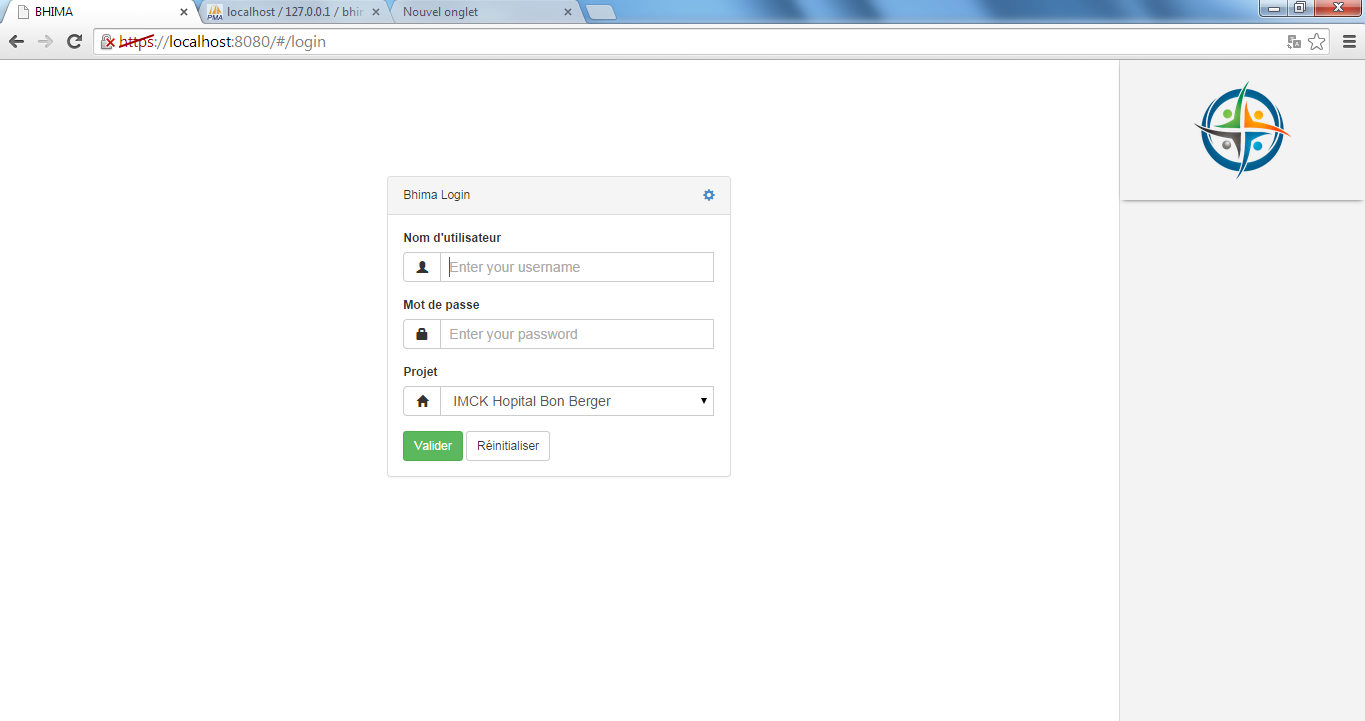
\includegraphics[width=12cm]{pic/login.png}
\end{center}
\caption{Page d'identification et authentification des utilisateurs}
\label{Page d'identification et authentification des utilisateurs}
\end{figure}
\\ L'accès au système n'est garanti que pour ceux qui possèdent un compte utilisateur, si l'utilisateur s'est authentifié alors il sera dirigé vers l'interface principale de l'application qui se présente de la manière suivante.
\newpage
\begin{figure}[h]
\begin{center} 
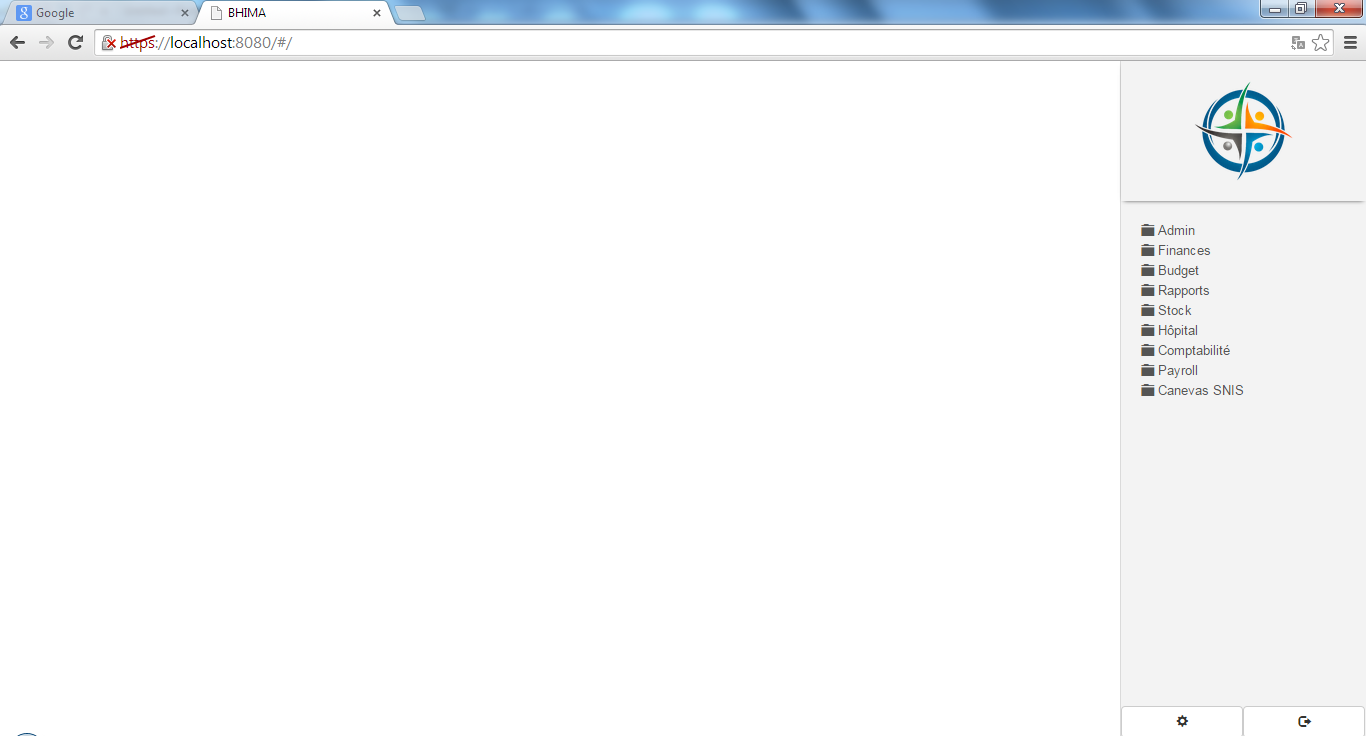
\includegraphics[width=10cm]{pic/mainInterface.png}
\end{center}
\caption{Interface principale de l'application}
\label{Interface principale de l'application}
\end{figure} 
Dans sa partie gauche de la figure ci-dessous on retrouve le logo IMA World Heath Ainsi que l'arborescence qui représente les modules du système auxquels l'utilisateur à accès. En dessous de l'arborescence figure deux boutons, le premier 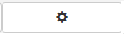
\includegraphics[scale=0.5]{pic/lang.png} permet de changer de langue et le second 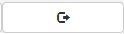
\includegraphics[scale=0.5]{pic/logout.png} permet de ce déconnecté du système.

\begin{figure}[h]
\begin{center}
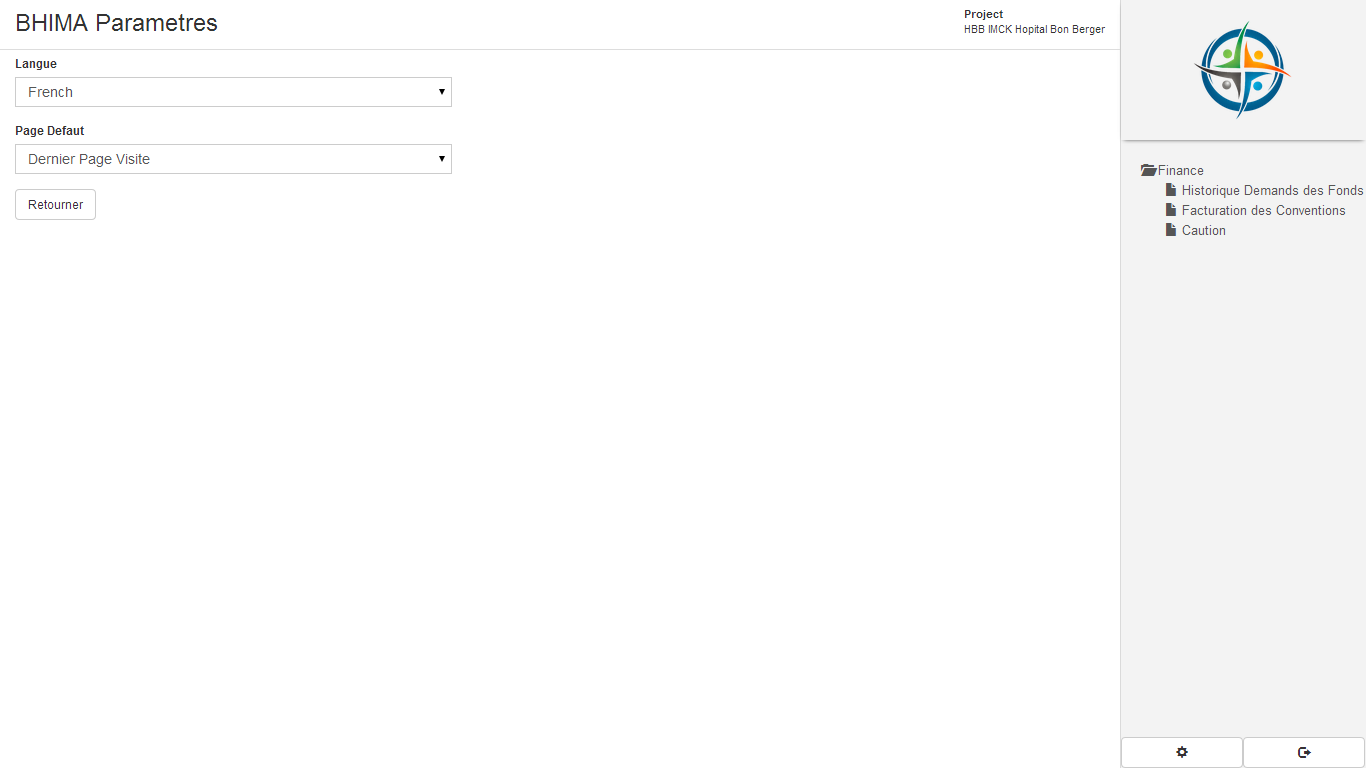
\includegraphics[width=10cm]{pic/changeLang.png}
\end{center}
\caption{Interface principale pour le changement de langue}
\label{Interface principale pour le changement de langue}
\end{figure} 

\section{Utilisation de l'arborescence de navigation}
L'arborescence de navigation contient les liens de chague module de l'application. Les modules sont regroupés en fonction de de leurs fonctionalités dans des dossiers tels que le dossier "Admin" affiché ci-dessous. Dans la première image, le dossier est fermé, en occultant tous les sous modules de ce module. Après le dossier est cliqué, une image d'un dossier ouvert montre que les contenus sont accessibles.

\begin{figure}[h]
\begin{center}
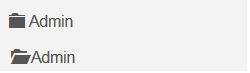
\includegraphics[width=4.5cm]{pic/folder_open_closed.png}
\end{center}
\caption{Etat d'un module ouvert et fermé}
\label{Etat d'un module ouvert et fermé}
\end{figure} 

Cliquant sur le dossier permet d'afficher la liste de sous modules sélectionné par l'utilisateur. Par exemple, ci-dessous, le dossier "Admin" est cliqué dans la premier illustration dans la séconde est ouverte tous ses sous modules.

\begin{figure}[h]
\begin{center}
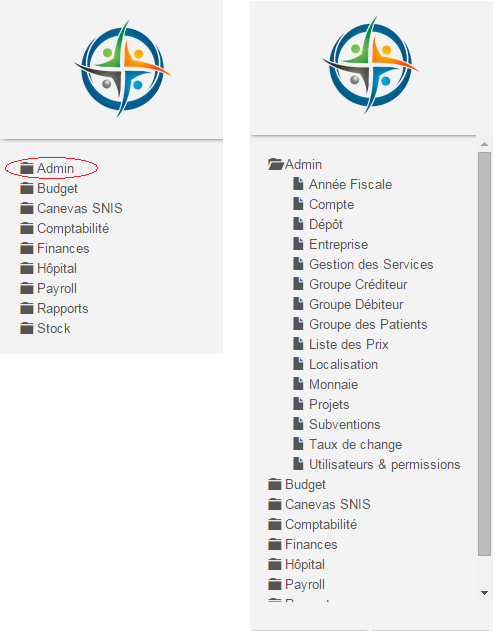
\includegraphics[width=8cm]{pic/open_folder.png}
\end{center}
\caption{Clique sur le dossier "admin" afin de pouvoir visualiser ses sous modules}
\label{Clique sur le dossier "admin" afin de pouvoir visualiser ses sous modules}
\end{figure} 


\newpage
\section{Les modules du système BHIMA}
Le système d'information BHIMA possède plusieurs modules qui sont représenté par l'arborescence ci-dessous.
\begin{figure}[h]
\begin{center}
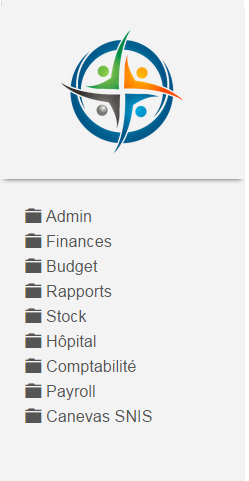
\includegraphics[width=4.5cm]{pic/arbo.png}
\end{center}
\caption{Arborescence du système}
\label{Arborescence du système}
Voici les différentes rubriques qui existent dans le système:
\end{figure} 
% Liste des modules
\begin{itemize}
\item Admin. %•
\item Budget
\item Canevas SNIS
\item Comptabilité
\item Finances
\item Hôpital
\item Payroll
\item Rapports
\item Stock
\end{itemize}


\newpage
%%%%%%%%%%%%%%%%%%%%%%%%%%%%%%%%%%%%%%%%%%%%%
%   MODULES DU SYSTEMES                     %
%%%%%%%%%%%%%%%%%%%%%%%%%%%%%%%%%%%%%%%%%%%%%
    
\chapter{Le module Admin}        
%////////////////////////////////////////////////%
% MODULE ADMIN
Le module admin est composé des sous modules qui permettent d'administrer le système. La figure ci-dessous représente avec exactitude ce module avec ses différents sous éléments.
\begin{figure}[h]
\begin{center}
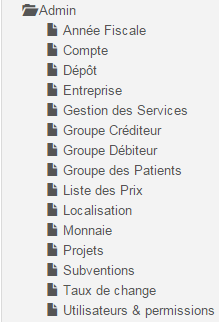
\includegraphics[width=4cm]{pic/s_admin.png}
\end{center}
\caption{Le module Admin et ses sous modules}
\label{Le module Admin et ses sous menus}
\end{figure} 


\section{Gestions des dépôts}
Ce menu permet d'enregistré mais aussi de gérer les dépôts.

\begin{figure}[h]
\begin{center}
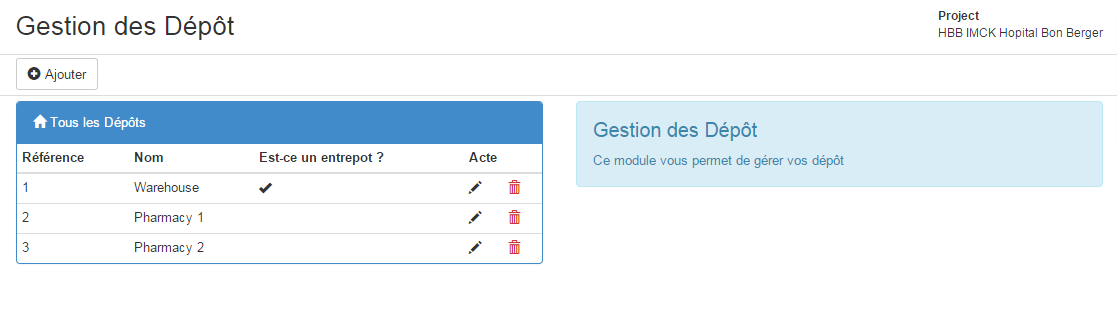
\includegraphics[width=14cm]{pic/GestionDesDepot.png}
\end{center}
\caption{Interface principale permetant la gestion des dépôts}
\label{Interface principale permetant la gestion des dépôts}
\end{figure}

Dans la partie gauche l'on trouve un bouton qui permet d'ajouter un nouveau dépôt. Pour ajouter un nouveau dépôt, il suffit de cliquer sur le bouton 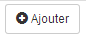
\includegraphics[scale=0.7]{pic/AddNewStore.png}.

\begin{figure}[h]
\begin{center}
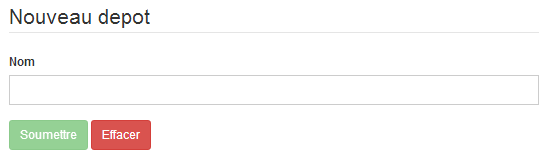
\includegraphics[width=10cm]{pic/NewStore.png}
\end{center}
\caption{Formulaire permettant d'ajouter un dépôt}
\label{Formulaire permettant d'ajouter un dépôt}
\end{figure}

Le formulaire ci-haut apparait lorsqu'un utilisateur clique sur le bouton \textbf{Ajouter}. Ce formulaire possède le champ \textbf{Nom} qui permet d'attribuer un nom à un dépôt, la case à cocher est ce un entrepôt permet de spécifier si le dépôt qui est entrain d'être enregistrer sera la principale dans l'organisation.
L'enregistrement est effectif seulement si l'utilisateur clique sur le bouton Soumettre. \textbf{La liste de tous les dépôts} apparait sous forme de tableau. Ce tableau afficher toutes les informations relatives entre autre le numéro de référence, le nom et La zone \textbf{Acte} renferme deux icônes le premier 
\includegraphics[scale=0.7]{pic/EditUser.png}  permet de modifier le nom d'un dépôt le second 
\includegraphics[scale=0.7]{pic/DeleteWRed.png}  permet de supprimer un dépôt.
\newpage


\newpage
\chapter{Le module Rapports}        
%////////////////////////////////////////////////%
Le module rapports permet de pouvoir visualiser plusieurs types des rapports résultants du fonctionnements du système, La figure ci-dessous représente avec exactitude ce module avec les différents sous éléments.

\begin{figure}[h]
\begin{center}
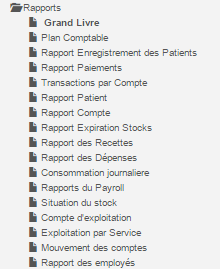
\includegraphics[width=4cm]{pic/ArboReport.png}
\end{center}
\caption{Arborescence du module Rapports}
\label{Arborescence du module Rapports}
\end{figure}

\newpage
\section{Rapport des commandes d'achat}
Le rapport de confirmation des commandes d'achat permet de visualiser l'historique de confirmation de commande d'achatdans le système. L'interface principale permettant de voire le rapport d'enregistrement des patients se présente de la manière suivante. 

\begin{figure}[h]
\begin{center}
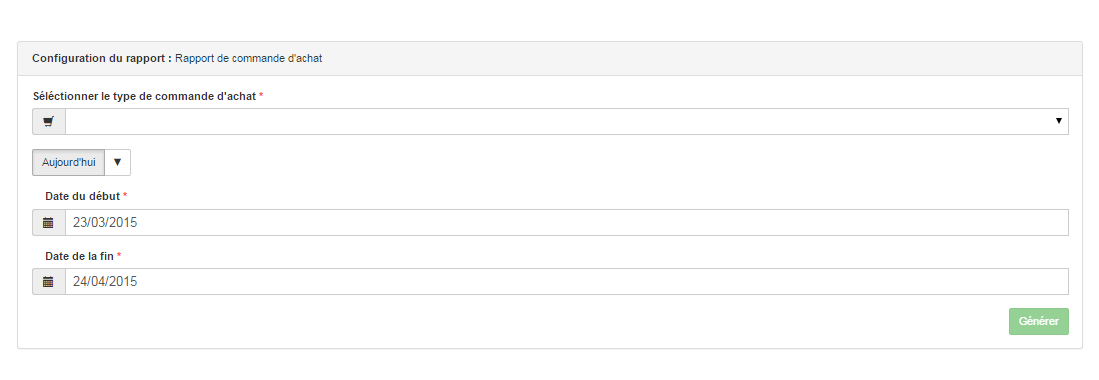
\includegraphics[width=10cm]{pic/RapConfPO.png}
\end{center}
\caption{Aperçue de l'interface principale du rapport de confirmation des commandes d'achat}
\label{Aperçue de l'interface principale du rapport de confirmation des commandes d'achat}
\end{figure}


La première zone permet de sélectionner le type de commande pour lequel on voudriai visualiser le rapport d'enregistrement, il y'a aussi une zone qui permet de spécifier l'écheance temporelle  ou bien spécifier directement la date du début et celle de la fin de la recherche. 

Le bouton générer permet l'affichage du tableau du rapport de confirmation de commande d'achat. L'interface permettant de visualier le rapport se présente de la manière suivante. Au dessus on retrouve deux boutons. le prémier 
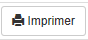
\includegraphics[scale=0.7]{pic/Print.png} permet d'imprimer le rapport et le second 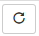
\includegraphics[scale=0.7]{pic/refresh.png} permet de faire une nouvelle recherche.

\begin{figure}[h]
\begin{center}
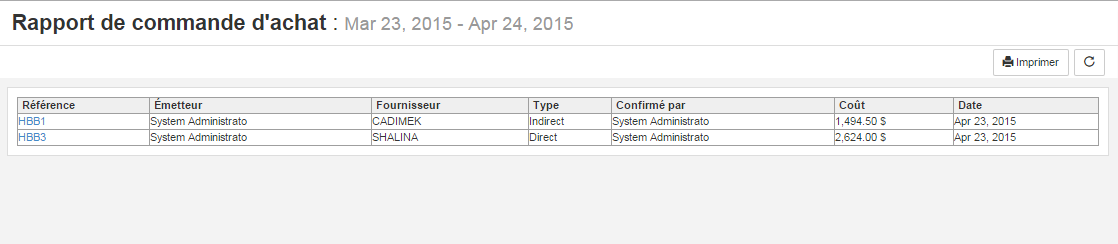
\includegraphics[width=12cm]{pic/RapportCommAchat.png}
\end{center}
\caption{Aperçue du résultat du rapport de confirmation des commandes d'achat}
\label{Aperçue du résultat du rapport de confirmation des commandes d'achat}
\end{figure}

\newpage
\section{Confirmation des donations}
Le rapport de Confirmation des donations permet de visualiser l'historique de confirmation Confirmation des donations dans le système. L'interface principale permettant de voire le rapport d'enregistrement des patients se présente de la manière suivante. 

\begin{figure}[h]
\begin{center}
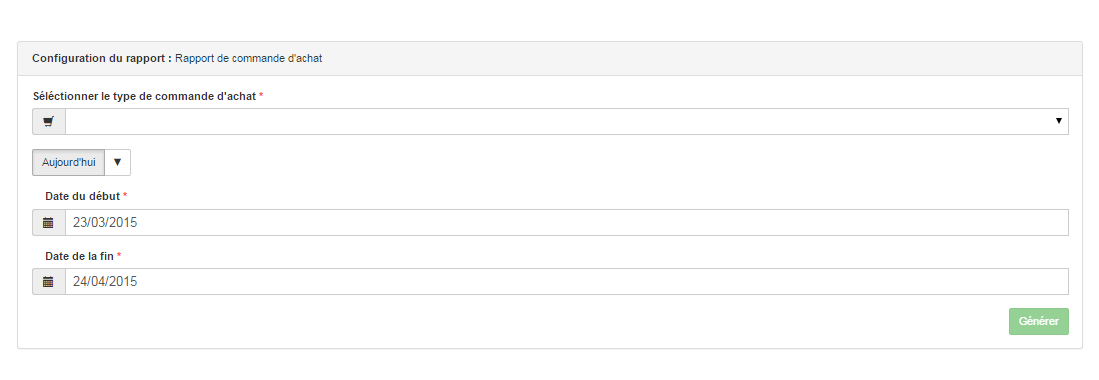
\includegraphics[width=10cm]{pic/RapConfPO.png}
\end{center}
\caption{Aperçue de l'interface principale du rapport de Confirmation des donations}
\label{Aperçue de l'interface principale du rapport de Confirmation des donations}
\end{figure}


La première zone permet de spécifier l'écheance temporelle  ou bien spécifier directement la date du début et celle de la fin de la recherche. 

Le bouton générer permet l'affichage du tableau du rapport de confirmation Confirmation des donations. L'interface permettant de visualier le rapport se présente de la manière suivante. Au dessus on retrouve deux boutons. le prémier 
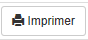
\includegraphics[scale=0.7]{pic/Print.png} permet d'imprimer le rapport et le second 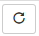
\includegraphics[scale=0.7]{pic/refresh.png} permet de faire une nouvelle recherche.

\begin{figure}[h]
\begin{center}
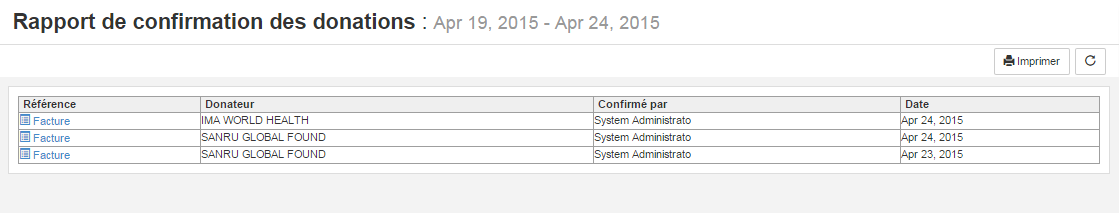
\includegraphics[width=12cm]{pic/RapConfDon.png}
\end{center}
\caption{Aperçue du résultat du rapport de confirmation des donations}
\label{Aperçue du résultat du rapport de confirmation des donations}
\end{figure}

\newpage
\section{Consommation journalière}
Le module consommation journalière permet de lister la consommation journalière des produits pharmaceutiques dans le système.
son interface principale se présente de la manière suivante.

\begin{figure}[h]
\begin{center}
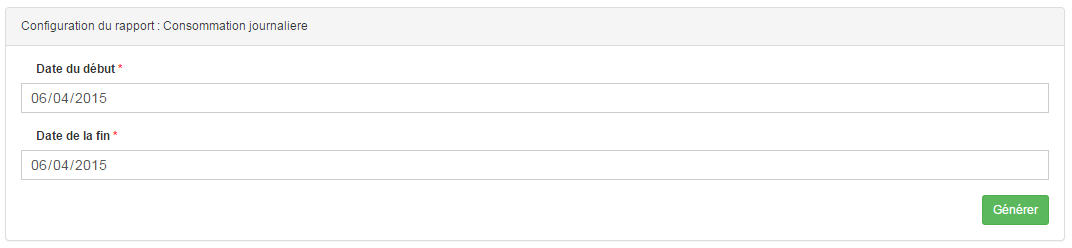
\includegraphics[width=14cm]{pic/ConsJour.png}
\end{center}
\caption{Interface principale du module consommation journalière}
\label{Interface principale du module consommation journalière}
\end{figure}

La figure ci haute est une illustration l'interface principale de la consommation journalière, cette interface permet de sélectionner la plage de temps pour laquelle on voudrait visualiser le rapport de la consommation. 

Le bouton générer permet l'affichage du tableau du rapport de la consommation journalière.
L'interface permettant de visualier le rapport se présente de la manière suivante. Au dessus on retrouve deux boutons. le prémier 
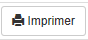
\includegraphics[scale=0.7]{pic/Print.png} permet d'imprimer le rapport et le second 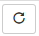
\includegraphics[scale=0.7]{pic/refresh.png} permet de faire une nouvelle recherche.

Le tableau du rapport de la consommation possède trois entête Code, Médicaments et Quantité total. Le code du médicament est un lien hypertexte qui permet une rédirection vers un autre rapport qui détaille la consommation effective d'un médicament par jour. 

\begin{figure}[h]
\begin{center}
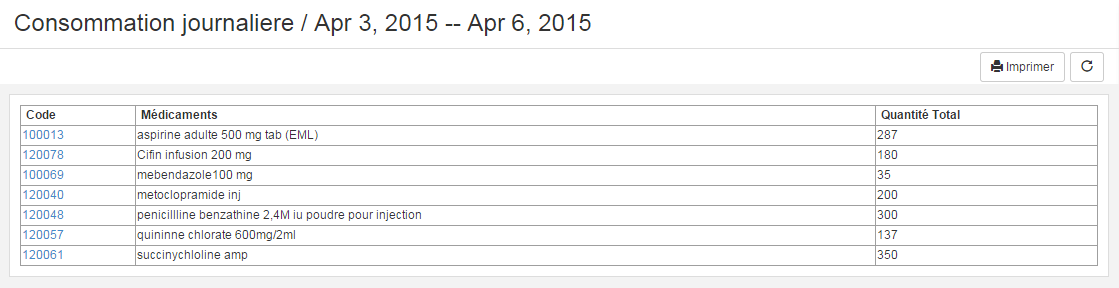
\includegraphics[width=14cm]{pic/ConsoJournProd.png}
\end{center}
\caption{Apperçue du Consommation journalière}
\label{Apperçue du Consommation journalière}
\end{figure}


La figure ci-après donne un apperçue du rapport de consommation journalière d'un produit par jour.

\begin{figure}[h]
\begin{center}
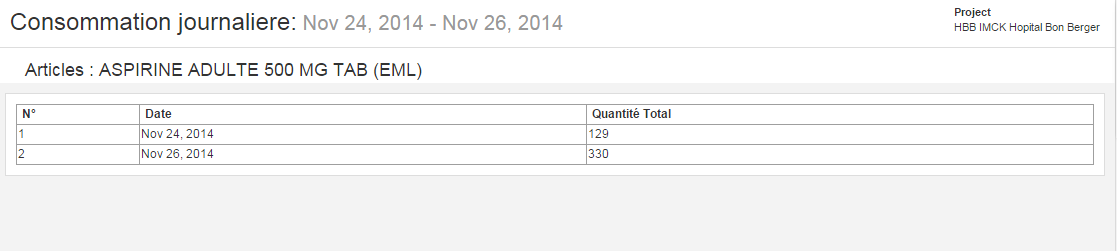
\includegraphics[width=14cm]{pic/ConsoDetJourn.png}
\end{center}
\caption{Apperçue de la consommation détaillée d'un produit}
\label{Apperçue de la consommation détaillée d'un produit}
\end{figure}


\newpage
\section{Historique des distributions aux patients}
Le module historique des distributions aux patients, permet de visualiser la consommation en produits pharmaceutiques des patients dans une plage de temps données.

L'interface principale de ce module se présente de la manière suivante

\begin{figure}[h]
\begin{center}
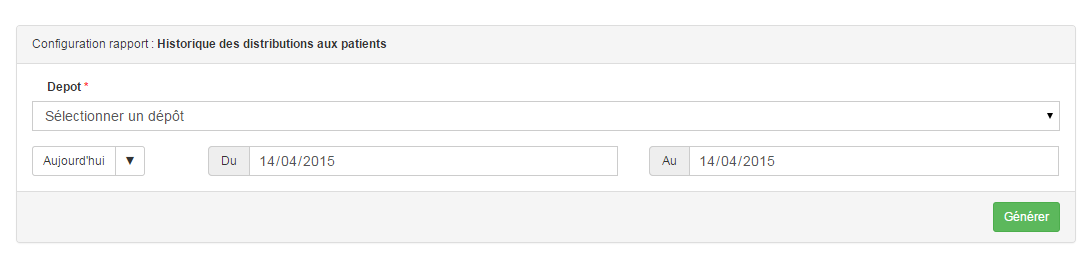
\includegraphics[width=14cm]{pic/HistDistrPatient.png}
\end{center}
\caption{Interface principale du module Historique des distributions aux patients}
\label{Interface principale du module Historique des distributions aux patients}
\end{figure}

L'interface permet de sélectionner le dépôt ainsi que la plage de temps pour laquelle on voudriai visualiser le rapport. 

Le bouton générer permet l'affichage du tableau du rapport Historique des distributions aux patients.
L'interface permettant de visualier le rapport se présente de la manière suivante. Au dessus on retrouve deux boutons. le prémier 
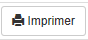
\includegraphics[scale=0.7]{pic/Print.png} permet d'imprimer le rapport et le second 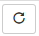
\includegraphics[scale=0.7]{pic/refresh.png} permet de faire une nouvelle recherche.

\begin{figure}[h]
\begin{center}
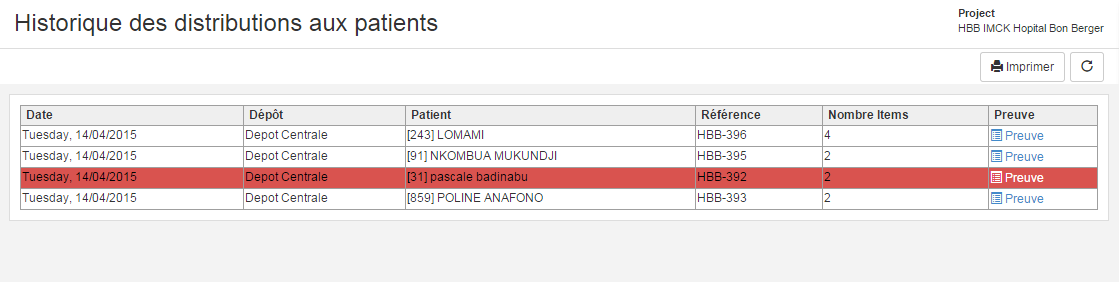
\includegraphics[width=14cm]{pic/TabHistDistPatient.png}
\end{center}
\caption{Rapport Historique des distributions aux patients}
\label{Rapport Historique des distributions aux patients}
\end{figure}

Les consommations annulées pour une raison ou une autre se démarque des autres avec une colorations en rouge. La colonne preuve donne la possibilité de pouvoir de revoir les différents éléments faisant partie de la consommation.

\newpage
\section{Historique des distributions aux services}
Le module historique des distributions aux services, permet de visualiser la consommation en produits pharmaceutiques des patients dans une plage de temps données.

L'interface principale de ce module se présente de la manière suivante

\begin{figure}[h]
\begin{center}
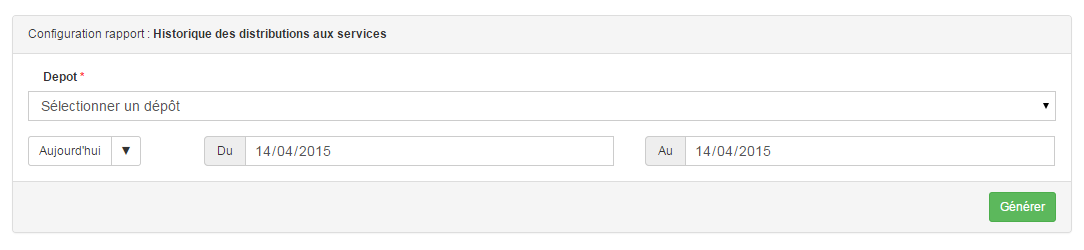
\includegraphics[width=14cm]{pic/HistDistServices1.png}
\end{center}
\caption{Interface principale du module Historique des distributions aux services}
\label{Interface principale du module Historique des distributions aux services}
\end{figure}

L'interface permet de sélectionner le dépôt ainsi que la plage de temps pour laquelle on voudriai visualiser le rapport. 

Le bouton générer permet l'affichage du tableau du rapport Historique des distributions aux services.
L'interface permettant de visualier le rapport se présente de la manière suivante. Au dessus on retrouve deux boutons. le prémier 
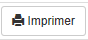
\includegraphics[scale=0.7]{pic/Print.png} permet d'imprimer le rapport et le second 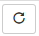
\includegraphics[scale=0.7]{pic/refresh.png} permet de faire une nouvelle recherche.

\begin{figure}[h]
\begin{center}
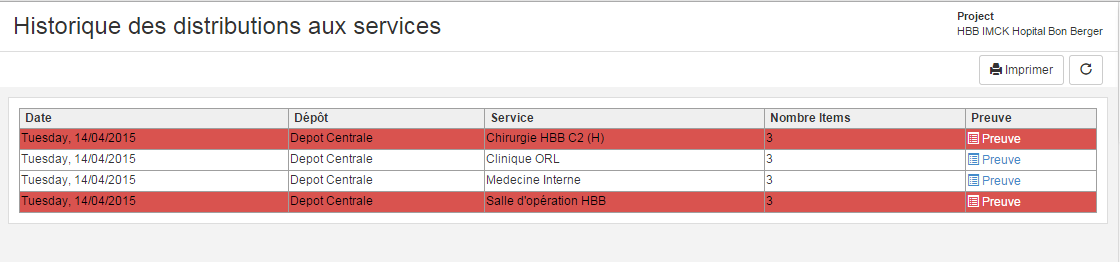
\includegraphics[width=14cm]{pic/tabHistDistServices.png}
\end{center}
\caption{Rapport Historique des distributions aux services}
\label{Rapport Historique des distributions aux services}
\end{figure}

Les consommations annulées pour une raison ou une autre se démarque des autres avec une colorations en rouge. La colonne preuve donne la possibilité de pouvoir de revoir les différents éléments faisant partie de la consommation.


\newpage
\section{Rapport d'expiration Stocks}
Le rapport Expiration Stocks permet d'avoir un brèf apperçue sur la péremption des produits pharmaceutiques, l'interface principale de ce module se présente de la manière suivante.

\begin{figure}[h]
\begin{center}
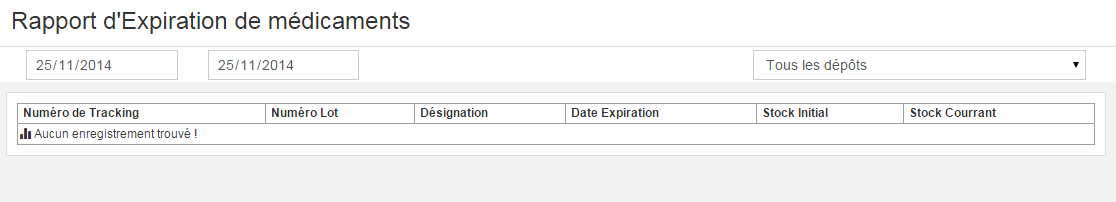
\includegraphics[width=10cm]{pic/RappExMedi.png}
\end{center}
\caption{Interface principale du module Rapport Expiration Stocks}
\label{Interface principale du module Rapport Expiration Stocks}
\end{figure}

La première zone permet de sélectionner le dépôt pour lequel on voudriai visualiser le rapport de péremption, il y'a aussi une zone qui permet de spécifier directement la date du début et celle de la fin de la recherche. 

Le bouton générer permet l'affichage du tableau du rapport d'expiration de stock. L'interface permettant de visualier le rapport se présente de la manière suivante. Au dessus on retrouve deux boutons. le prémier 
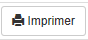
\includegraphics[scale=0.7]{pic/Print.png} permet d'imprimer le rapport et le second 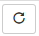
\includegraphics[scale=0.7]{pic/refresh.png} permet de faire une nouvelle recherche.

\begin{figure}[h]
\begin{center}
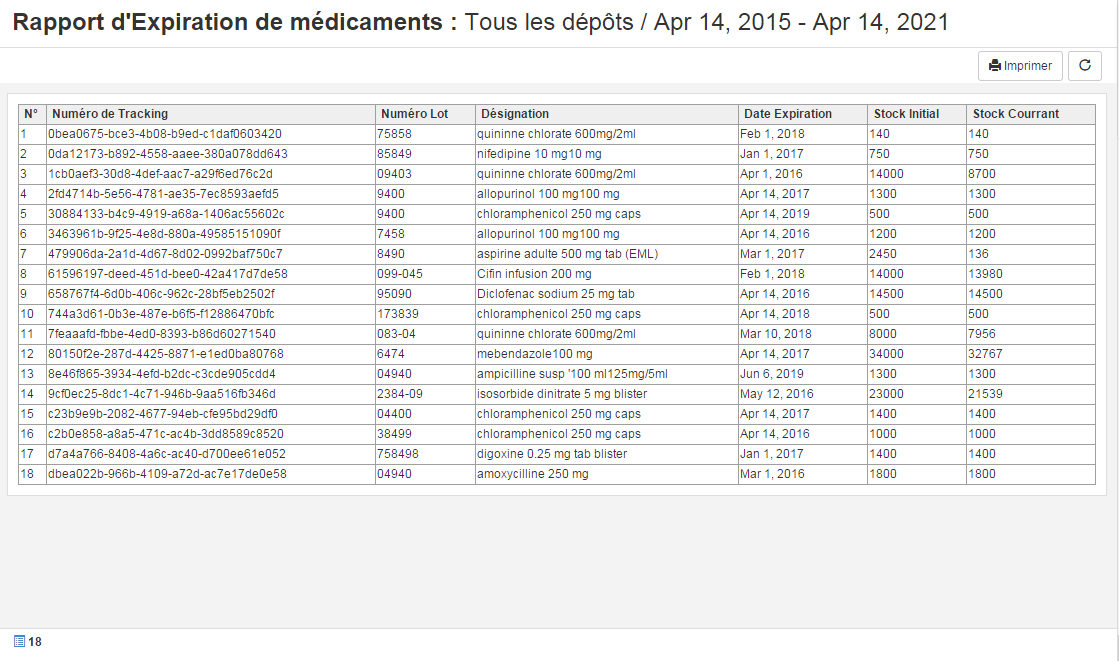
\includegraphics[width=12cm]{pic/AppRapExMedi.png}
\end{center}
\caption{Aperçue du résultat du rapport d'expiration des produits pharmaceutiques}
\label{Aperçue du résultat du rapport d'expiration des produits pharmaceutiques}
\end{figure}

\newpage
\section{Rapport de pertes de stock}
Le rapport de pertes de stock permet de visualiser l'historique de pertes de stock, qu'ils s'agissent de vol des produits, de la perte, de la peremption ainsi que de la déterioration des produits. L'interface principale permettant de voire le rapport de pertes de stock se présente de la manière suivante. 

\begin{figure}[h]
\begin{center}
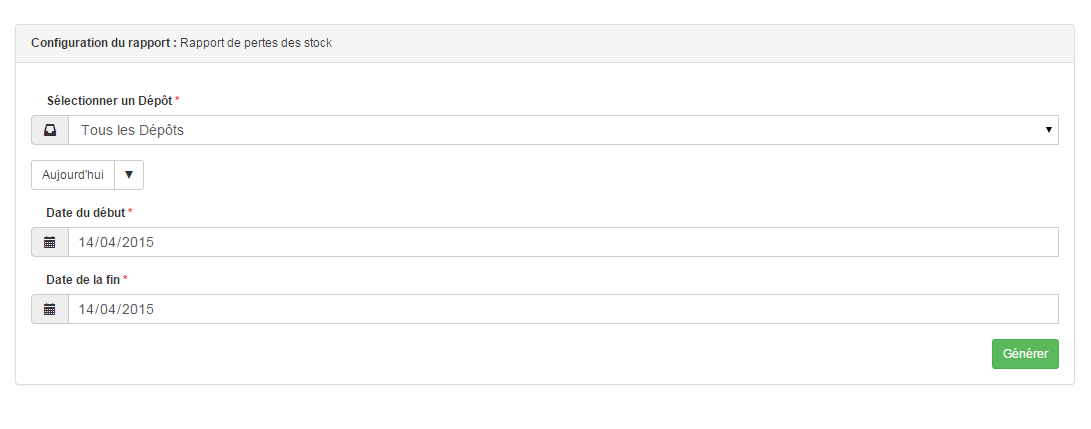
\includegraphics[width=10cm]{pic/ConfPerStock.png}
\end{center}
\caption{Aperçue de l'interface principale du rapport de pertes de stock}
\label{Aperçue de l'interface principale du rapport de pertes de stock}
\end{figure}


La première zone permet de sélectionner le dépôt pour lequel on voudriai visualiser le rapport de pertes de stock, il y'a aussi une zone qui permet de spécifier l'écheance temporelle  ou bien spécifier directement la date du début et celle de la fin de la recherche. 

Le bouton générer permet l'affichage du tableau du rapport de pertes de stock. L'interface permettant de visualier le rapport se présente de la manière suivante. Au dessus on retrouve deux boutons. le prémier 
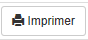
\includegraphics[scale=0.7]{pic/Print.png} permet d'imprimer le rapport et le second 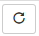
\includegraphics[scale=0.7]{pic/refresh.png} permet de faire une nouvelle recherche.


\begin{figure}[h]
\begin{center}
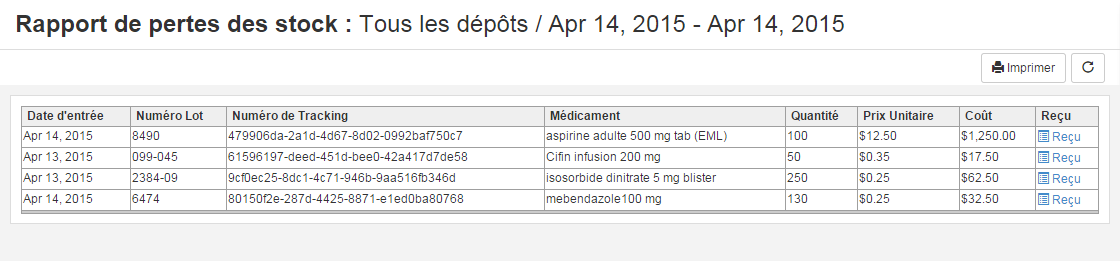
\includegraphics[width=12cm]{pic/PerteStockRapport.png}
\end{center}
\caption{Aperçue du résultat du rapport de perte des stock}
\label{Aperçue du résultat du rapport de perte des stock}
\end{figure}

\newpage
\section{Rapport des donations}
Le rapport des donations permet de visualiser l'historique de toutes les donations effectuer par un donateur spécifique, l'interface pricipale se présente de manière suivante. 

\begin{figure}[h]
\begin{center}
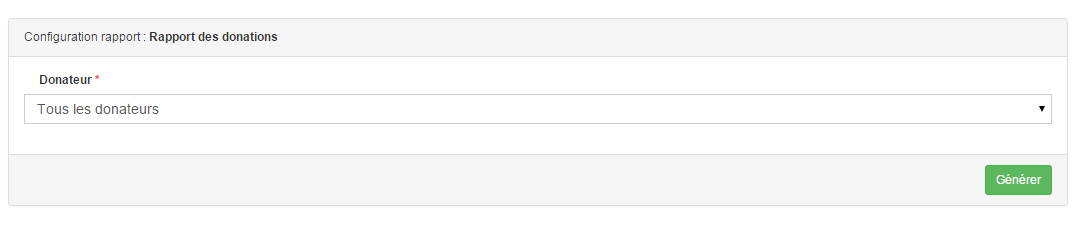
\includegraphics[width=10cm]{pic/RapDonnInterface.png}
\end{center}
\caption{Aperçue de l'interface principale du rapport des donations}
\label{Aperçue de l'interface principale du rapport des donations}
\end{figure}


Il n'existe qu'une seule zone, celle ci permet de sélectionner directement un donateur dans la liste des donateurs enregistrées. Le bouton générer permet l'affichage du tableau du rapport des donations. L'interface permettant de visualier le rapport se présente de la manière suivante. Au dessus on retrouve deux boutons. le prémier 
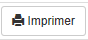
\includegraphics[scale=0.7]{pic/Print.png} permet d'imprimer le rapport et le second 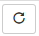
\includegraphics[scale=0.7]{pic/refresh.png} permet de faire une nouvelle recherche.


\begin{figure}[h]
\begin{center}
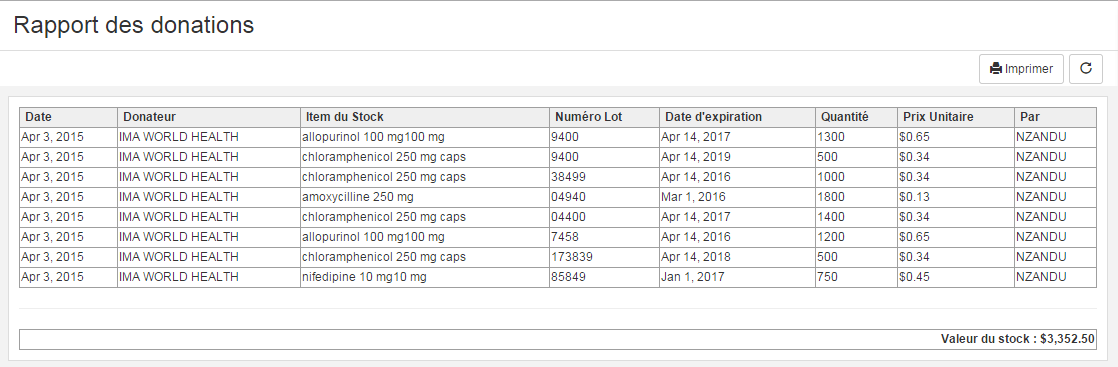
\includegraphics[width=14cm]{pic/DonationsRapport.png}
\end{center}
\caption{Aperçue du résultat du rapport des donations}
\label{Aperçue du résultat du rapport des donations}
\end{figure}


\newpage
\section{Situation de stock}
le rapport de situation de stock permet de faire le contrôle de l'inventaire, le module de situation de stock utilise le système de revue continue ou permanente, aussi appelé système de commande à intervalle variable. dans ce système le niveau de stock est revisé sur une base permanente pour chague transaction effectuée sur le stock. Lorsque le stock atteint un niveau déterminé pour le réapprovisionnement, une commande doit être faite. Ce système est basé sur les niveaux de stock plutôt que sur les intervalles de temps.

L'interface principale de ce module se présente de la manière suivante.

\begin{figure}[h]
\begin{center}
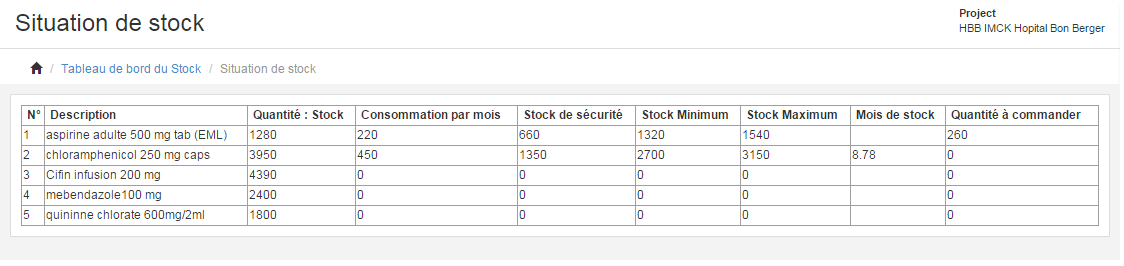
\includegraphics[width=14cm]{pic/SituationStock.png}
\end{center}
\caption{Interface principale du Situation de stock}
\label{Interface principale du Situation de stock}
\end{figure}

Le tableau représentant la situation en stock comporte différent colonnes, ces colonnes comportes des données permettant l'établissement des niveaux de stock adéquats pour surmonter les fluctuations et les incohérences de livraison, les responsables peuvent établir un niveau d'inventaire maximum et minimum.

Voici les différents colonnes qui apparaisent dans le tableau de la situation de stock:
\begin{itemize}
\item Description. 
\item Quantité en stock
\item Consommation par mois
\item Stock de sécurité
\item Stock minimum
\item Stock maximum
\item Mois de stock
\item Quantité à commander
\end{itemize}

\subsection{Description}
La colonne description renseigne sur le nom commercial du produit pharmaceutique ainsi que le type d'emballage qui le categorise.

\subsection{Quantité en stock}
La quantité en stock renseigne sur le niveaux de stock du produit dans le différent dépôt, la quantité en stock ne renseigne pas les stocks qui a était distribuer aux services.

\subsection{Consommation par mois}
La consommation moyenne corresponds à la consommation moyenne mensuelle d'un produit durant le six dernier mois de la consommation, la consommation moyenne mensuelle ne tient pas compte des produits qui sont perdus ou abimés ou bien perimés et ne considere pas non plus les périodes de rupture de stock mais seulement de ceux qui ont été réelement consommés.

\subsection{Stock de sécurité}
Le stock de sécurité correspond à la réserve utilisée pour prévenir les ruptures de stock consécutives à des livraisonns tardives, à des ruptures de stock de produits au niveau du fournisseur, ou à l'utilisation du stock à un niveau élevé imprévisiblement. Le niveau du stock de sécurité requis est généralement différent pour chaque programme et doit être basé sur les données de la consommation établies dans le passé.

L'obtention du stock de sécurité s'effectue en multipliant la consommation moyenne mensuelle de six dernier mois de la consommation par le delai de livraison moyenne entre la période de commande et de livraison d'un médicament.

Dans la plupart de cas le stock de sécurité doit au moins être plus important que celui d'une période de revision afin de repondre à des demandes accrues ou de faire face à des livraisons tardives imprévues. 

\subsection{Stock minimum}
Le niveau de stock minimum est le niveau en déça duquel les stocks ne doivent jamais descendre sans qu'une commande ne soit faite. C'est la quantité du stock à utiliser pendant la période entre la commande et la réception du produit en plus d'une réserve ou stock de sécurité pour faire face aux urgences, et aux demandes non prevues ainsi qu'aux livraison tardives.

L'obtention du stock minimum s'effectue en multipliant le stock minimum par deux.

\subsection{Stock maximum}
Le niveau de stock maximum permet de prévenir les sur-approvisionnements qui entrainent la perte des produits en raison de leur péremption avant qu'ils ne puissent être distribués.

L'obtention du stock maximum s'effectue en multipliant la consommation moyenne mensuelle de six dernier mois par l'intervalle de commande et ensuite additionner au produit le niveau de stock minimum.

\subsection{Mois de stock}
Le mois de stock est une autre façon d'exprimer le stock en termes des nombres des mois d'approvisionnement disponibles en stock. le nombre de mois en stock permet de prevenir dans combien des mois un produis doit être réapprovisionner afin d'éviter que le stock initial soit en deçà de son niveau minimum.
Le mois de stock est le rapport entre niveau de stock d'un produit par la niveau de la consommation moyenne mensuelle de six dernier mois. 

\subsection{Quantité à commander}
La quantité à commander optimale à utilisé pour chaque produits lors de l'établissement des ordres d'achat, cette quantité est obtenue en établissant la différence entre le niveau de stock maximum d'un produit avec le niveau en stock.



\newpage
\chapter{Stock}        
%////////////////////////////////////////////////%
Le module Stock est composé des sous modules qui permettent d'administrer le stock. La figure ci-dessous représente avec exactitude ce module avec ses différents sous éléments.

\begin{figure}[h]
\begin{center}
\includegraphics[width=6cm]{pic/StockManagement.png}
\end{center}
\caption{Arborescence du module Stock}
\label{Arborescence du module Stock}
\end{figure}


\section{Enregistrement des fournisseurs}
Le module Enregistrement des fournisseurs permet de faire l'enregistrement des fournisseurs.

\begin{figure}[h]
\begin{center}
\includegraphics[width=14cm]{pic/InterEnrFourn.png}
\end{center}
\caption{Interface principale du module enregistrement des fournisseurs}
\label{Interface principale du module enregistrement des fournisseurs}
\end{figure}

Dans la figure ci-haute on retrouve dans la partie supérieur gauche le bouton \textbf{Enregistrer fournisseur} qui permet de reafficher le formulaire d'enregistrement des fournisseurs, il y'a aussi le bouton \textbf{Créer un groupe créditeur} qui renvoi les utilisateurs vers le module d'ajout des groupes créditeur. Dans la partie moyenne on retrouve à gauche le formulaire d'enregistrement des fournisseurs et dans la partie droite la liste des fournisseurs incrits.

le formulaire d'enregistrement des fournisseurs nécessites pour l'enregistrement d'un fournisseur les éléments ci-après: Son nom, son groupe créditeur, son numéro de téléphone, son adresse e-mail, sa localisation géographique ainsi qu'un certain nombre d'information optionnelles, l'enregistrement est effective que si l'on clique sur le bouton \includegraphics[scale=0.7]{pic/CreatSupplier.png}.

Le tableau permet de lister les fournisseurs inscrits possède le bouton \includegraphics[scale=0.7]{pic/EditSupplier.png} qui permet d'afficher le formulaire de mise à jour des informations liées à un fournisseur, une fois que les modifications sont faites il existe en bas du formulaire le bouton \includegraphics[scale=0.7]{pic/MettreJourSuppl.png} qui permet de sauvegarder les données mis à jour.
\newpage

\section{Gestion des donateurs}
Le module gestion des donateurs est un module qui a été conçu pour permettre l'administration des différents donateurs de l'organisation, le tableau qui se trouve à gauche permet d’enregistrer, de mettre à jour les attributs d'un donateur ainsi que la suppression.
\begin{figure}[h]
\begin{center}
\includegraphics[width=14cm]{pic/GestionDonateur.png}
\end{center}
\caption{Interface principale de la gestion des donateurs}
\label{Interface principale de la gestion des donateurs}
\end{figure}

Dans la figure ci-haute on retrouve dans la partie gauche la liste des différents donateurs enregistrés dans le système, au dessus de ce tableau existe le bouton \includegraphics[scale=1]{pic/AddDonor.png} qui permet d'ajouter un nouveau donateur dans le système, le formulaire permettant de faire l'enregistrement de donateur se présente de la manière suivante.

\begin{figure}[h]
\begin{center}
\includegraphics[width=8cm]{pic/NewDonor.png}
\end{center}
\caption{Formulaire permettant l'enregistrement des donateurs}
\label{Formulaire permettant l'enregistrement des donateurs}
\end{figure} 

Le formulaire permettant l'enregistrement des donqteurs est très simple, il ne contient que la zone de saisie permettant de renseigner le nom du donateur, et l'enregistrement est effective que si l'on clique sur le bouton soumettre. 

Les tableaux réprésentant les fonctions enregistrées donne la possibilité de pouvoir mettre à jour les informations rélative à un donateur, dans la zone action de ce tableau on retrouve deux icônes, l'icône \includegraphics[scale=0.7]{pic/EditBlack.png} qui permet de mettre à jour une fonction et \includegraphics[scale=0.7]{pic/DeleteWRed.png} permet de supprimer une fonction dans le système.
Voici un apperçu du formulaire permettant la mise à jour des informations d'un fonction, la mise à jour est effective que si l'on modifier les informations dont on a besoin en validant grace au bouton soumettre. 

\begin{figure}[h]
\begin{center}
\includegraphics[width=8cm]{pic/UpdateDonor.png}
\end{center}
\caption{Formulaire permettant de mettre à jour un donateur}
\label{Formulaire permettant de mettre à jour un donateur}
\end{figure} 


\newpage
\section{Gestion de l'Inventaire}
Le module gestion de l'inventaire permet d'administrer les inventaires existant dans le système. Grace à ce module il est possible d'enregistrer les articles, les mettre à jour, faire la configurations des groupes d'articles, de configurer les différents types qui existent, de voire la liste des articles existant ainsi que la possibilité d'imprimer les articles existant.

Voici l'interface principale du module permettant de faire la gestion des inventaires.

\begin{figure}[h]
\begin{center}
\includegraphics[width=12cm]{pic/GestInventaires.png}
\end{center}
\caption{Menu principale de la gestion des inventaires}
\label{Menu principale de la gestion des inventaires}
\end{figure}

\subsection{Enregistrer Article}
Le module enregistrer article permet d'enregistrer les différents articles existant dans le système. son interface principale se présente de la manière suivante.

\begin{figure}[h]
\begin{center}
\includegraphics[width=12cm]{pic/SaveStock.png}
\end{center}
\caption{Interface principale de l'enregistrement des inventaires}
\label{Interface principale de l'enregistrement des inventaires}
\end{figure}

Dans la partie gauche de la figure ci-haute on retrouve la zone \textbf{Général} qui possede un formulaire qui permet de spécifier le type d'inventaire qu'il faut enregistrer, de donner une codification de l'article, ainsi que sa description mais aussi de spécifier dans quelle groupe d'inventaire faira partie la nouvelle article. 

Dans la partie droite on retrouve la zone \textbf{Informations pour la Facturation et Stocks} qui possède un autre formulaire qui fait suite au précedant et qui permet de spécifier si l'inventaire est un produit durable ou non. Il existe une liste de choix \textbf{Unit} qui permet de determiner la nature unitaire de l'inventaire, mais aussi des zones de saisie permettant d'enregistrer le prix d'achat, le prix de vente, le poid unitaire ainsi que le volume unitaire de l'inventaire. Après avoir renseigné tous ses élements le bouton \textbf{Soumettre} permet de l'enregistrement effective de l'inventaire.


\subsection{Mettre à jour Article}
Le module mettre à jour un article permet de modifier les informations rélatives à un article. l'interface principale de ce module est doté d'une zone de recheche qui permet de rechercher tous les articles enregistrés dans le système.
La figure ci-dessous représente l'interface principale de ce module.

\begin{figure}[h]
\begin{center}
\includegraphics[width=14cm]{pic/EditInventaire.png}
\end{center}
\caption{Interface principale permettant de mettre à jour d'un inventaire}
\label{Interface principale permettant de mettre à jour d'un inventaire}
\end{figure}
\newpage
La zone de recherche de ce module fonctionne comme un filtre, et losqu'on a trouvé l'article dont on veut apporter des modification, il suffit de cliquer sur le bouton \textbf{Soumettre} pour pouvoir voire les informations rélatives à cet article. Voici un apperçue de la mise à jour d'un article.

\begin{figure}[h]
\begin{center}
\includegraphics[width=14cm]{pic/GestInventareUpdt.png}
\end{center}
\caption{Apperçue du processus de mis à jour d'un inventaire}
\label{Apperçue du processus de mis à jour d'un inventaire}
\end{figure}

Dans la partie gauche de l'image ci haut on retrouve la zone réserver à l'historique du prix de vente de l'article, dans la partie qui se touve à gauche ont retrouve toutes les autres informations rélatives à l'article, pour effectuer une opération des mis à jour il suffit de cliquer sur le bouton \textbf{Soumettre} pour valider la mis à jour. 

\newpage
\subsection{Configurer Groupes des Articles}
Le module configurer groupes permet d'adminsitrer les différents groupes d'articles existant au sein du système, ce module est doté des interfaces permettant l'enregistrement ainsi que la mis à jour des groupes d'articles. L'interface principale de ce module fonctionne de la manière suivant.

\begin{figure}[h]
\begin{center}
\includegraphics[width=10cm]{pic/GroupeMedicament.png}
\end{center}
\caption{Interface principale permettant la configuration de groupe d'article}
\label{Interface principale permettant la configuration de groupe d'article}
\end{figure}

On retrouve dans le coin supérieur droite le bouton \includegraphics[scale=0.7]{pic/CreerGroupeArticle.png} qui permet d'afficher le formulaire permettant de faire l'enregistrement de groupe d'articles, le formulaire permettant l'enregistrement de groupe d'article se présente de la manière suivante.

\begin{figure}[h]
\begin{center}
\includegraphics[width=10cm]{pic/AddGroupStock.png}
\end{center}
\caption{Formulaire permettant l'enregistrement de groupe d'article}
\label{Formulaire permettant l'enregistrement de groupe d'article}
\end{figure}

Pour enregistrer un groupe d'article il faudrait spécifier le nom du groupe, le code de l'article, le numéro de compte de \textbf{Produit ou bien de Profit}, le numéro de compte de \textbf{Charge}, le numéro du compte de \textbf{Stock} ansi que le numéro de stock de donation. Une fois que toutes ces informations sont renseignés, il suffit de cliquer sur le bouton \textbf{Sauver Changement} pour enregistrer le nouveau groupe d'article.

Dans la partie gauche de l'interface d'adminstration de groupe de Stock on retrouve le tableau des différents groupes des stock existant dans le système. Le tableau des groupes de stock possède des entêtes dont l'une d'elle intitulé \textbf{Action} possède une petite icône \includegraphics[scale=0.7]{pic/EditBlack.png} qui permet d'afficher l'interface qui permet de faire la mis à jour des informations rélatives à un groupe de stock. 

Le formulaire permettant de faire la mise à jour des informations permettant de faire la mise à jour est très similaire à celui permettant l'enregistrement d'un groupe de stock, mais à la différence que celui affiche les informations rélatives à un groupe de stock dans chacune des zones de saisie correspondante, et la mis à jour n'est effective que si après modification des informations existantes on clique sur le bouton \textbf{Sauver Changement}.


\subsection{Configurer Type d'Articles}
Le module configurer type d'article permet d'adminsitrer les différents types d'articles existant au sein du système, ce module est doté des interfaces permettant l'enregistrement ainsi que la mis à jour des types d'articles. L'interface principale de ce module fonctionne de la manière suivant.

\begin{figure}[h]
\begin{center}
\includegraphics[width=10cm]{pic/GesTypesArticle.png}
\end{center}
\caption{Interface principale permettant la configuration de type d'article}
\label{Interface principale permettant la configuration de type d'article}
\end{figure}

On retrouve dans le coin supérieur droite le bouton \includegraphics[scale=0.7]{pic/AddnewType.png} qui permet d'afficher le formulaire permettant de faire l'enregistrement de type d'article, le formulaire permettant l'enregistrement de type d'article se présente de la manière suivante.

\begin{figure}[h]
\begin{center}
\includegraphics[width=10cm]{pic/FormAddTypeArt.png}
\end{center}
\caption{Formulaire permettant l'enregistrement de type d'article}
\label{Formulaire permettant l'enregistrement de type d'article}
\end{figure}

Pour enregistrer un type d'article il faudrait spécifier tout simplement le nom du type et de cliquer sur le bouton \textbf{Soumettre} pour enregistrer le nouveau type d'article.

Dans la partie gauche de l'interface d'adminstration de type d'article on retrouve le tableau des différents types d'articles existant dans le système. Le tableau possède deux entêtes texte et \textbf{Action} ce dernier possède une petite icône \includegraphics[scale=0.7]{pic/EditBlack.png} qui permet d'afficher l'interface qui permet de faire la mis à jour des informations rélatives à un type d'article. 

Le formulaire permettant de faire la mise à jour des informations relative à un type d'article est très similaire à celui permettant l'enregistrement mais à la différence que celui affiche les informations rélatives à un type d'article dans une zone de saisie, et la mis à jour n'est effective que si après modification des informations existantes on clique sur le bouton \textbf{Soumettre}.

\newpage
\subsection{Voire la liste}
Le module voire la liste permet de lister tous les articles enregistrés. son interface principale possède deux boutons en entête le premier \textbf{Groupé par} permet de faire plusieurs type de groupement par rapport à la présentation de la liste des articles et le second \textbf{Enregistrer stock} permet une redirection vers le formulaire permettant de faire l'enregistrement des articles dans la base de données. L'interface principale permettant de ce module se présente de la manière suivante.

\begin{figure}[h]
\begin{center}
\includegraphics[width=10cm]{pic/JournalStock.png}
\end{center}
\caption{Interface principale du module voire liste}
\label{Interface principale du module voire liste}
\end{figure}

Les entêtes de ce tableau permet de faire le trie des élements de la colonne cliquer de manière ascendante et descendanr,le bouton \textbf{Groupé par} propose plusieurs façon de regrouper les articles, la figure suivante donne un aperçue des différents types regroupements que propose ce module.

\begin{figure}[h]
\begin{center}
\includegraphics[width=4cm]{pic/GroupeParItem.png}
\end{center}
\caption{Apperçue des différents types des regroupements}
\label{Apperçue des différents types des regroupements}
\end{figure}

\newpage
Voici un apperçue de la liste des articles avec un regroupement fait sur le critaire du prix de vente.

\begin{figure}[h]
\begin{center}
\includegraphics[width=10cm]{pic/GroupPrice.png}
\end{center}
\caption{Apperçue du regroupement par prix de vente}
\label{Apperçue du regroupement par prix de vente}
\end{figure}

\newpage
\subsection{Imprimer la liste des Articles}
Le module imprimer la liste des articles permet de l'affichage de la liste de tous les articles enregistrés dans le système ainsi que la possibilté de faire l'impressionde cette liste grace au bouton \includegraphics[scale=0.7]{pic/Imprint.png}.

\begin{figure}[h]
\begin{center}
\includegraphics[width=14cm]{pic/manifInventaire.png}
\end{center}
\caption{Apperçue de l'interface permettant de faire l'impression de la liste des articles}
\label{Apperçue de l'interface permettant de faire l'impression de la liste des articles}
\end{figure}

\newpage
\section{Gestion des commandes d'achats}
Le module gestion des commandes d'achats permet d'administrer tous les processus d'approvisionement en stock, en commançant par l'établissement de la commande d'achat. Le menu principale permettant la gestion des ordres d'achat se présente de la manière suivante.

\begin{figure}[h]
\begin{center}
\includegraphics[width=14cm]{pic/GestOrdAchat.png}
\end{center}
\caption{Menu principale de gestion des commandes d'achat}
\label{Menu principale de gestion des commandes d'achat}
\end{figure}

\subsection{Créer une commande d'achat}
Le module de création de commande d'achat est doté d'une interface permettant de spécifier toutes les informations rélatives à une commande, son interface principale se présente de la manière suivante.

\begin{figure}[h]
\begin{center}
\includegraphics[width=12cm]{pic/OrdreAchatForm.png}
\end{center}
\caption{Apperçue du formulaire permettant de créer une commande}
\label{Apperçue du formulaire permettant de créer une commande}
\end{figure}

Le formulaire permettant permettant de créer une commande d'achat a dans sa partie gauche réserver au paramètrage, donne la possibilité de pouvoir spécifier le type de commande à établir ansi que la séléction de la date de la commande d'achat, très important pour certain module.

Dans le cas d'une commande d'achat indirect il est necessaire de pouvoir spécifier le fournisseur ainsi que de l'employé responsable de la livraison ainsi que le nom de l'achateur mais dans le cas d'une commande d'achat direct il n'est pas nécessaire de spécifier un achateur car celle-ci s'éffectue directement entre l'entreprise et le fournissaire via les transactions bancaires. Une fois que les données de paramètrage sont déterminer, la zone commande d'achat retranscri ses éléments dans un tableau.

En bas de page existe une zone permettant de choisir les produits qui feront partie d'une commande d'achat comme le montre la figure suivante.

\begin{figure}[h]
\begin{center}
\includegraphics[width=12cm]{pic/ItemsOrdonnees.png}
\end{center}
\caption{Apperçue de la zone permettant de choisir les produits faisant partie d'une commande d'achat}
\label{Apperçue de la zone permettant de choisir les produits faisant partie d'une commande d'achat}
\end{figure} 

Pour pouvoir chercher un produit il faudrai le faire dans \includegraphics[scale=0.4]{pic/SearchInventory.png} la zone qui fonctionne comme un filtre, ensuite preciser la quantité, le prix d'achat. Si l'on veux ajouter un autre produit, il suffit de cliquer sur le bouton \includegraphics[scale=0.7]{pic/AjArticleGreen.png}.

Une fois que la sélection les produits est effectuée le bouton \includegraphics[scale=0.7]{pic/SunPurchaseOrder.png} permet de valider la création d'une commande d'achat.

Voici un aperçue des spécimens de commande d'achat générée automatiquement les systèmes.

\begin{figure}[h]
\begin{center}
\includegraphics[width=12cm]{pic/OrdreAchatInvoice.png}
\end{center}
\caption{Apperçu d'une commande d'achat indirecte}
\label{Apperçu d'une commande d'achat indirecte}
\end{figure}  

\begin{figure}[h]
\begin{center}
\includegraphics[width=12cm]{pic/ComAchatDirect.png}
\end{center}
\caption{Apperçu d'une commande d'achat directe}
\label{Apperçu d'une commande d'achat directe}
\end{figure}

\textbf{NB} Après avoir créer une commande d'achat celle ci devrait être validée et authorisé par la hièrachie.
\newpage
\subsection{Liste des commandes d'Achats}
Le module liste des commandes d'achat archive tous les commandes d'achat qui ont étaient effectué dans le système. Ces commandes d'achat se présente sous forme d'un tableau et donne la possibilité de pouvoir revoire le détail d'une commande d'achat. Son interface principale se présente de la manière suivante..

\begin{figure}[h]
\begin{center}
\includegraphics[width=12cm]{pic/ListeOrdreAchat.png}
\end{center}
\caption{Interface principale du module liste des commandes d'achat}
\label{Interface principale du module liste des commandes d'achat}
\end{figure} 

Dans l'entête de cette zone on retrouve une zone de recherche fonctionnant comme un filtre et à sa droite il y'a le bouton recherche avancé.
En dessous de la zone d'entête on retrouve le tableau des archives des commandes d'achat, les commandes d'achat qui ont été déjà confirmé ont dans la colonne \textbf{Payé} l'icône \includegraphics[scale=0.7]{pic/OkCOnfPOrd.png} et ceux qui sont en entête de paiement possède l'icône \includegraphics[scale=0.7]{pic/OrConKO.png} . Pour visualiser les détails d'une commande d'achat il suffit de cliquer sur le bouton \includegraphics[scale=0.7]{pic/VoirDetail.png} qui permet une redirection vers la page qui permet de la faire. 

\newpage
\section{Confirmation des Commande d'achats}
Le module Confirmation des Commande d'achats permet de confirmer le paiement de la commande d'achat ainsi que l'acquisition des produits concernés par cette commande d'achat. L'interface principale de ce module se présente de la manière suivante.

\begin{figure}[h]
\begin{center}
\includegraphics[width=12cm]{pic/ConfPaieAchat.png}
\end{center}
\caption{Interface principale du module Confirmation des Commande d'achats}
\label{Interface principale du module Confirmation des Commande d'achats}
\end{figure}  

Dans la partie gauche de ce module ont retrouve par défaut la liste des commandes d'achat indirect en attente de confirmation mais il est possible de pouvoir afficher la liste de commande d'achat direct en attente de confirmation tout simplement en cochant le bouton \textbf{Direct}. Au dessus du tableau listant les commandes d'achat ont retrouve, une petite zone de recherche qui fonctionne comme un filtre qui permer de rechercher les commandes d'achat à partir de leur référence.

Pour confirmer une commande d'achat il suffit de cliquer sur le bouton \includegraphics[scale=0.7]{pic/BlueArrow.png} pour pouvoir afficher les informations rélatives de cette commande d'achat. La figure ci après illustre bien le processus de confirmation de paiement d'une commande d'achat, il existe en dessous des informations rélatives à une commande d'achat le bouton de confirmation  de la commande avec le nom de la personne qui a été responsable du paiement.

\begin{figure}[h]
\begin{center}
\includegraphics[width=12cm]{pic/ConfPOAchat.png}
\end{center}
\caption{Apperçue du processus de confirmation d'une commande d'achat indirect}
\label{Apperçue du processus de confirmation d'une commande d'achat indirect}
\end{figure} 

\begin{figure}[h]
\begin{center}
\includegraphics[width=12cm]{pic/JustSonCaisse.png}
\end{center}
\caption{Apperçue de la Justificatif de bon de sortie caisse (Commande d'achat indirect)}
\label{Apperçue de la Justificatif de bon de sortie caisse  (Commande d'achat indirect)}
\end{figure} 

\newpage

\begin{figure}[h]
\begin{center}
\includegraphics[width=12cm]{pic/ConfPOAchatDirect.png}
\end{center}
\caption{Apperçue du processus de confirmation d'une commande d'achat direct}
\label{Apperçue du processus de confirmation d'une commande d'achat direct}
\end{figure} 


\begin{figure}[h]
\begin{center}
\includegraphics[width=12cm]{pic/ConfComAchat.png}
\end{center}
\caption{Apperçue de la note de Confirmation Commande d'achat(Commande d'achat direct)}
\label{Apperçue de la note de Confirmation Commande d'achat(Commande d'achat direct)}
\end{figure} 

\newpage
\section{Confirmation Donation}
Le module Confirmation des donationspermet de confirmer l'entrée en stock effective des produits provenant d'un don. L'interface principale de ce module se présente de la manière suivante.

\begin{figure}[h]
\begin{center}
\includegraphics[width=12cm]{pic/ConfPaieAchat.png}
\end{center}
\caption{Interface principale du module Confirmation des Commande d'achats}
\label{Interface principale du module Confirmation des Commande d'achats}
\end{figure}  

Dans la partie gauche de ce module ont retrouve par défaut la liste des dons qui n'ont pas encore étaient confirmés. Au dessus du tableau listant les donations on retrouvent, une petite zone de recherche qui fonctionne comme un filtre qui permer de rechercher les donations à partir de leur référence.

Pour confirmer une donation il suffit de cliquer sur le bouton \includegraphics[scale=0.7]{pic/BlueArrow.png} pour pouvoir afficher les informations rélatives de cette donation. La figure ci après illustre bien le processus de confirmation d'une donation, il existe en dessous des informations rélatives à une donation, le bouton de confirmation  de la donation avec le nom du donateur.

\begin{figure}[h]
\begin{center}
\includegraphics[width=12cm]{pic/ConfirDonation.png}
\end{center}
\caption{Apperçue du processus de confirmation d'une donation}
\label{Apperçue du processus de confirmation d'une donation}
\end{figure} 

\begin{figure}[h]
\begin{center}
\includegraphics[width=12cm]{pic/PreuveConfDonation.png}
\end{center}
\caption{Apperçue de la Justificatif de Confirmation de la donation}
\label{Apperçue de la Justificatif de Confirmation de la donation}
\end{figure} 


\newpage
\section{Tableau de bord du Stock}
Le tableau de bord du stock est une interface permettant de visualiser plus informations rélative à la gestion des stock. L'interface principale de ce module se présente de la manière suivante.

\begin{figure}[h]
\begin{center}
\includegraphics[width=12cm]{pic/TaBordStock.png}
\end{center}
\caption{Interface principale du Tableau de bord du stock}
\label{Interface principale du Tableau de bord du stock}
\end{figure} 

Le tableau de bord de stock permet de renseigner sur les 10 meilleurs produits les plus consommés, il s'agit pour cela des toutes les distributions des produits au près des patients et au près des services. 

le tableau de bord permet aussi de renseigner sur l'état des commandes qui ont eu lieu en renseignant sur:
\begin{itemize}
\item les nombres des commandes d'achat qui ont était effectué mais qui n'ont pas encore était payé (en attente de paiement);
\item les nombres des commandes d'achat pour les quels la caisse principale a effectué les paiements (payés);
\item les nombres des commandes pour lesquels il n' y a pas encore eu d'entrée en stock (en attente de reception);
\item les nombres des commandes pour lesquels il n' y a eu effectivement entrée en stock (reçues);
\end{itemize}

Le tableau de bord donne aussi des informations du stock par produits, on peut ainsi connaitre le nombre des produits qui sont en ruptire des stock, le nombres des produits pour lesquels la quantité existante est en dessous de la quantité minimal optimal en stock , ceux qui ont une quantité supérieur à la quantité maximal optimum en stock mais aussi le nombre de ceux dont la quantité en stock est optimale.

Le tableau de bord donne aussi un apperçue sur la péremption des médicaments en indiquant les nombres des produits encore en stock et qui ont expirés, ainsi que plusieurs échéances d'expiration des médicaments et les nombres des produits rélative en chacun d'entre eux.

Le tableau de bord renseigne aussi sur les produits qui ont étaient acquis grâce à des oeuvres des charités ou bien de dons, en listant les 10 derniers qui ont eu lieu dans un tableau qui permet de connaitre le nom du donateur ainsi que la date de la donation.

Le tableau de bord permet de sa rubrique rapports d'avoir un apperçue sur la situation glôbale en stock ainsi que sur la quantité des produits à risque de péremption.




%%%%%%%%%%%%%%%%%%%%%%%%%%%%%%%%%%%%%%%%%%%%%%%%%
% Table des matieres
\tableofcontents
\end{document}